\documentclass[12pt]{article}

%%%%%%%%%%%%%%%%%%%%%%%%%%%%%%%%%%%%%%%%%%%%%%%%%%%%%%%%%%%%%%%%%%%%%%%%%%%%%%%%%%%%%%%%%%%%%%%%%%%%
% Math
\usepackage{fancyhdr} 
\usepackage{amsfonts}
\usepackage{amsmath}
\usepackage{amssymb}
\usepackage{amsthm}
%\usepackage{dsfont}

%%%%%%%%%%%%%%%%%%%%%%%%%%%%%%%%%%%%%%%%%%%%%%%%%%%%%%%%%%%%%%%%%%%%%%%%%%%%%%%%%%%%%%%%%%%%%%%%%%%%
% Macros
\usepackage{calc}

%%%%%%%%%%%%%%%%%%%%%%%%%%%%%%%%%%%%%%%%%%%%%%%%%%%%%%%%%%%%%%%%%%%%%%%%%%%%%%%%%%%%%%%%%%%%%%%%%%%%
% Commands and Custom Variables	
\newcommand{\problem}[1]{\hspace{-4 ex} \large \textbf{Problem #1} }
\let\oldemptyset\emptyset
\let\emptyset\varnothing
\newcommand{\norm}[1]{\left\lVert#1\right\rVert}
\newcommand{\sint}{\text{s}\kern-5pt\int}
\newcommand{\powerset}{\mathcal{P}}
\renewenvironment{proof}{\hspace{-4 ex} \emph{Proof}:}{\qed}
\newcommand{\RR}{\mathbb{R}}
\newcommand{\NN}{\mathbb{N}}
\newcommand{\QQ}{\mathbb{Q}}
\newcommand{\ZZ}{\mathbb{Z}}
\newcommand{\CC}{\mathbb{C}}


%%%%%%%%%%%%%%%%%%%%%%%%%%%%%%%%%%%%%%%%%%%%%%%%%%%%%%%%%%%%%%%%%%%%%%%%%%%%%%%%%%%%%%%%%%%%%%%%%%%%
%page
\usepackage[margin=1in]{geometry}
\usepackage{setspace}
%\doublespacing
\allowdisplaybreaks
\pagestyle{fancy}
\fancyhf{}
\rhead{Shaw \space \thepage}
\setlength\parindent{0pt}

%%%%%%%%%%%%%%%%%%%%%%%%%%%%%%%%%%%%%%%%%%%%%%%%%%%%%%%%%%%%%%%%%%%%%%%%%%%%%%%%%%%%%%%%%%%%%%%%%%%%
%Code
\usepackage{listings}
\usepackage{courier}
\lstset{
	language=Python,
	showstringspaces=false,
	formfeed=newpage,
	tabsize=4,
	commentstyle=\itshape,
	basicstyle=\ttfamily,
}

%%%%%%%%%%%%%%%%%%%%%%%%%%%%%%%%%%%%%%%%%%%%%%%%%%%%%%%%%%%%%%%%%%%%%%%%%%%%%%%%%%%%%%%%%%%%%%%%%%%%
%Images
\usepackage{graphicx}
\graphicspath{ {images/} }
\usepackage{float}

%tikz
\usepackage[utf8]{inputenc}
\usepackage{pgfplots}
\usepgfplotslibrary{groupplots}

%%%%%%%%%%%%%%%%%%%%%%%%%%%%%%%%%%%%%%%%%%%%%%%%%%%%%%%%%%%%%%%%%%%%%%%%%%%%%%%%%%%%%%%%%%%%%%%%%%%%
%Hyperlinks
%\usepackage{hyperref}
%\hypersetup{
%	colorlinks=true,
%	linkcolor=blue,
%	filecolor=magenta,      
%	urlcolor=cyan,
%}

\begin{document}
	\thispagestyle{empty}
	
	\begin{flushright}
		Sage Shaw \\
		m527 - Fall 2017 \\
		\today
	\end{flushright}
	
{\large \textbf{HW 10}}\bigbreak

%%%%%%%%%%%%%%%%%%%%%%%%%%%%%%%%%%%%%%%%%%%%%%%%%%%%%%%%%%%%%%%%%%%%%%%%%%%%%%%%%%%%%%%%%%%%%%%%%%%%
\problem{1} Find the three cube roots of $64i$. \\

	\begin{align*}
		64i & = 64e^{\pi/2} = 64e^{-3\pi/2} = 64e^{5\pi/2} \\
		(64e^{\pi/2})^{1/3} & = 4(e^{\pi/2})^{1/3} \\
		& = 4(e^{\pi/6}) = 2\sqrt{3}+2i \\
		(64e^{-3\pi/2})^{1/3} & = 4(e^{-3\pi/2})^{1/3} \\
		& = 4(e^{-\pi/2}) = -4i \\
		(64e^{5\pi/2})^{1/3} & = 4(e^{5\pi/2})^{1/3} \\
		& = 4(e^{5\pi/6}) = -2\sqrt{3}+2i
	\end{align*}
	
	Thus 
	\begin{align*}
		4(e^{\pi/6}) &= 2\sqrt{3}+2i \\
		4(e^{-\pi/2}) &= -4i \\
		4(e^{5\pi/6}) &= -2\sqrt{3}+2i
	\end{align*}
	are the three cube roots of $64i$.
	\bigbreak

%%%%%%%%%%%%%%%%%%%%%%%%%%%%%%%%%%%%%%%%%%%%%%%%%%%%%%%%%%%%%%%%%%%%%%%%%%%%%%%%%%%%%%%%%%%%%%%%%%%%
{\hspace{-4 ex} \large \textbf{Section 13.3}}\bigbreak
\problem{\# 3} Determine and graph the set given by $\pi < \vert z - 4 + 2i \vert < 3\pi$. \bigbreak

	This is the set of points within the circle of radius $3\pi$ centered at $4-2i$ but outside of the circle of radius $\pi$ with the same center.
	
	\begin{figure}[H]
		%\caption{The plot of Cosine along with the degree 4 LS approximation and the error.}
		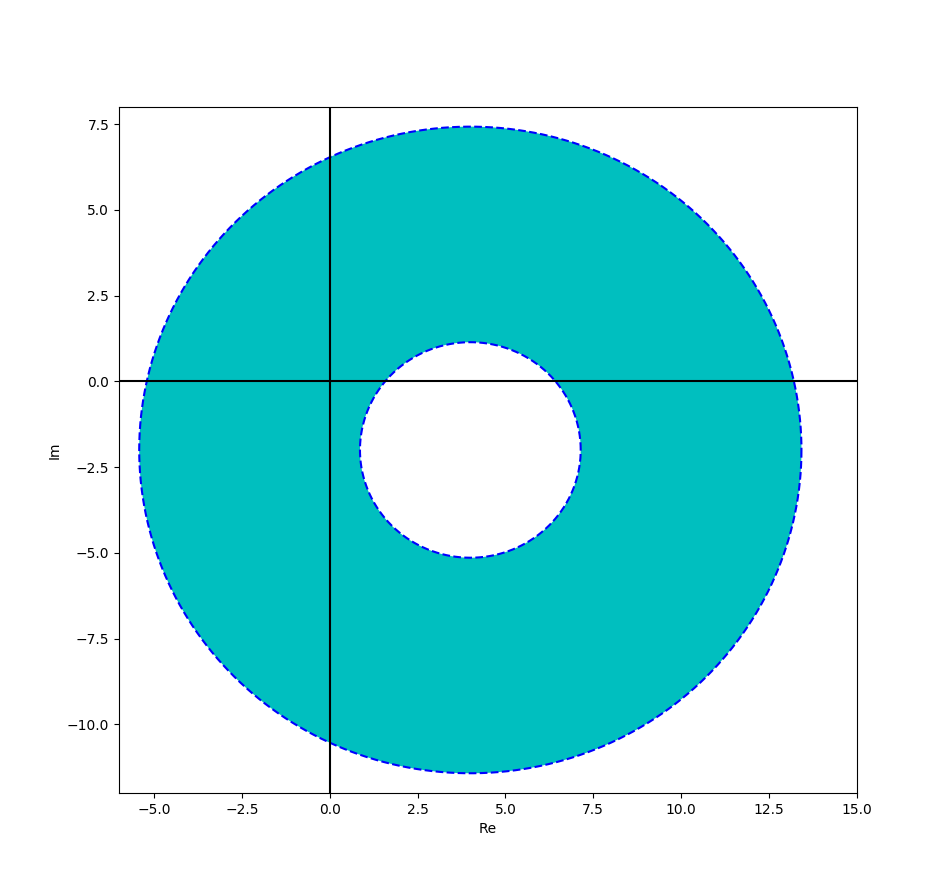
\includegraphics[width=0.75\textwidth]{hw10_figure_1}
		%\label{legendre_approx}
		\centering
	\end{figure}



\bigbreak
%%%%%%%%%%%%%%%%%%%%%%%%%%%%%%%%%%%%%%%%%%%%%%%%%%%%%%%%%%%%%%%%%%%%%%%%%%%%%%%%%%%%%%%%%%%%%%%%%%%%
\problem{\# 6}Determine and graph the set given by $\Re(1/z)<1$. \bigbreak

	\begin{align*}
		\Re(1/z) &< 1\\
		\Re(1/(x+iy)) &< 1\\
		\Re \Bigg(\frac{x-iy}{x^2+y^2} \Bigg) &< 1 \\
		\frac{x}{x^2+y^2} &< 1 \\
		x &< x^2 + y^2 \\
		0 &< x^2 - x + \tfrac{1}{4} - \tfrac{1}{4} + y^2 \\
		\tfrac{1}{4} &< (x-\tfrac{1}{2})^2 +y^2
	\end{align*}
	This describes the region outside the circle of radius $\tfrac{1}{2}$ centered at $\tfrac{1}{2} + 0i$.
	\begin{figure}[H]
		%\caption{The plot of Cosine along with the degree 4 LS approximation and the error.}
		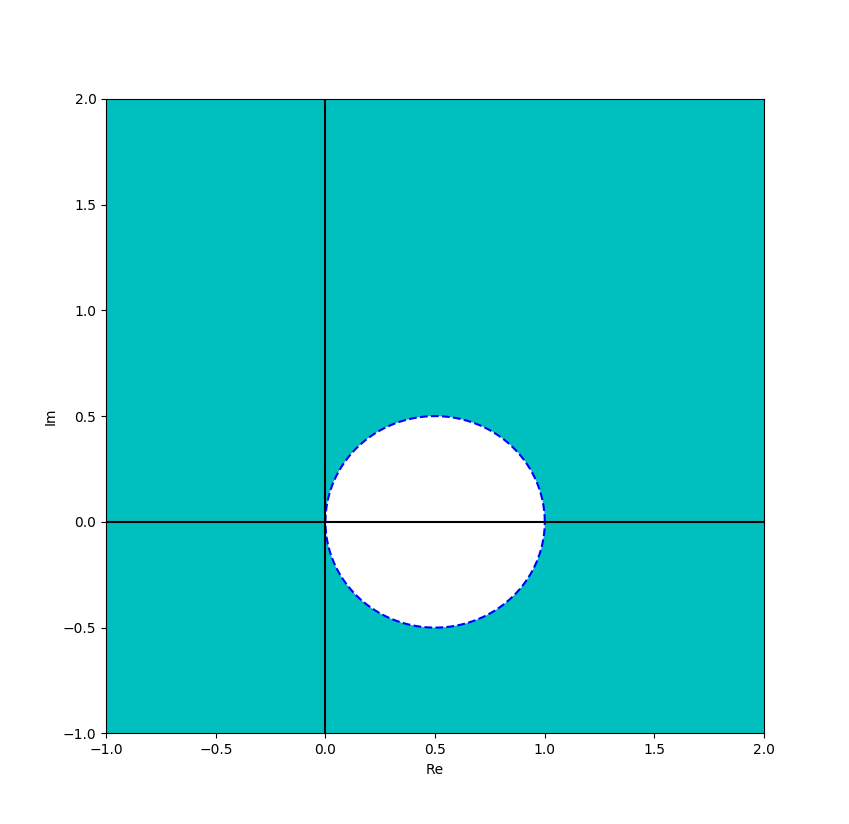
\includegraphics[width=0.75\textwidth]{hw10_figure_2}
		%\label{legendre_approx}
		\centering
	\end{figure}

\bigbreak
%%%%%%%%%%%%%%%%%%%%%%%%%%%%%%%%%%%%%%%%%%%%%%%%%%%%%%%%%%%%%%%%%%%%%%%%%%%%%%%%%%%%%%%%%%%%%%%%%%%%
\problem{\# 24e} Show that $f(z) = \Re(z)$ is not differentiable anywhere. Can you find other such functions?

\bigbreak
{\hspace{-4 ex} \large \textbf{Section 13.4}}\bigbreak
%%%%%%%%%%%%%%%%%%%%%%%%%%%%%%%%%%%%%%%%%%%%%%%%%%%%%%%%%%%%%%%%%%%%%%%%%%%%%%%%%%%%%%%%%%%%%%%%%%%%
\problem{\# 24}

\bigbreak
%%%%%%%%%%%%%%%%%%%%%%%%%%%%%%%%%%%%%%%%%%%%%%%%%%%%%%%%%%%%%%%%%%%%%%%%%%%%%%%%%%%%%%%%%%%%%%%%%%%%
\problem{4} Find all solutions of thte equation $\cos(z) = 4i$. \bigbreak

	\begin{align*}
		\cos(z) &= 4i \\
		\tfrac{1}{2}(e^{iz}+e^{-iz}) &= 4i \\
		e^{iz}+e^{-iz} &= 8i \\
		e^{2iz}+e^{0} &= 8ie^{iz} \\
		(e^{iz})^2 -8i e^{iz} + 1 & = 1 \\
		e^{iz} &= \frac{8i \pm \sqrt{-64 - 4}}{2} \\
		e^{iz} &= (4 \pm \sqrt{17})i \\
		e^{i(x+iy)} &= (4 \pm \sqrt{17})i \\
		e^{-y+xi} &= 0 + (4 \pm \sqrt{17})i \\
		e^{-y}\cos(x) + e^{-y}\sin(x)i &= 0 + (4 \pm \sqrt{17})i \\
	\end{align*}
	Since $e^{-y} \neq 0$, we can conclude that $\cos(x) = 0$ and thus $x = \tfrac{\pi}{2}+n\pi$ for $n \in \ZZ$. If $n$ is even then $\sin(x) = 1$ and 
	\begin{align*}
		e^{-y} & = (4 \pm \sqrt{17}) \\
		e^{-y} & = (4 + \sqrt{17}) \text{\ \ ($e^{-y}$ only assumes positive values)}\\
		y & = -\ln(4 + \sqrt{17})
	\end{align*} 
	If $n$ is odd, then $\sin(x) = -1$ and
	\begin{align*}
		-e^{-y} & = (4 \pm \sqrt{17}) \\
		-e^{-y} & = (4 - \sqrt{17}) \text{\ \ ($-e^{-y}$ only assumes negative values)}\\
		e^{-y} & = (\sqrt{17}-4) \text{\ \ ($-e^{-y}$ only assumes negative values)}\\
		y & = - \ln(\sqrt{17}-4)
	\end{align*}
	So $z = \tfrac{\pi}{2}+2m\pi -\ln(4 + \sqrt{17})i$ and $z = \tfrac{3\pi}{2}+2m\pi - \ln(\sqrt{17}-4)i$ where $m \in \ZZ$ are all of the values of $z$ such that $\cos(z) = 4i$.
	

\end{document}
